\section{得分函数估计}
\label{sec:pgrad-score}

上一节最后的两个例子里，样本沿生成路径的变化是跳跃式的，路径导数看不到期望的变化。还有一些情形根本没有方便的生成映射，例如样本由Markov链产生。这时可以换一个角度：不跟踪样本点怎样移动，而看各位置的概率权重怎样变化。参数改变时，有的位置质量增加，有的减少；把函数值按这种增减加权求和，就是期望的变化率。第~\ref{chap:information-geometry}章的得分函数正好记录了每个位置上质量的相对变化率。

本节先处理密度可以完整计算的情形，再处理只知道密度到一个随参数变化的常数因子的情形。

\subsection{已归一化密度}
\label{sec:pgrad-score-normalized}

设$P_{\bm{\theta}}$相对固定的参考测度$\nu$有密度$p_{\bm{\theta}}$，支撑$S=\{x:p_{\bm{\theta}}(x)>0\}$不随$\bm{\theta}$改变。在$S$上，得分函数是
\[
  \bm{s}_{\bm{\theta}}(x)=\nabla_{\bm{\theta}}\ln p_{\bm{\theta}}(x)=\frac{\nabla_{\bm{\theta}}p_{\bm{\theta}}(x)}{p_{\bm{\theta}}(x)} .
\]
把期望写成参考测度上的积分
\[
  J(\bm{\theta})=\int_{S}f_{\bm{\theta}}\,p_{\bm{\theta}}\,\mathrm{d}\nu,
\]
在定理~\ref{thm:pgrad-exchange}中取$\mu$为$\nu$在$S$上的限制，以乘积$f_{\bm{\theta}}p_{\bm{\theta}}$作$g$。乘积的导数是
\[
  \nabla_{\bm{\theta}}(f_{\bm{\theta}}p_{\bm{\theta}})=p_{\bm{\theta}}\nabla_{\bm{\theta}}f_{\bm{\theta}}+f_{\bm{\theta}}\nabla_{\bm{\theta}}p_{\bm{\theta}}=p_{\bm{\theta}}\bigl(\nabla_{\bm{\theta}}f_{\bm{\theta}}+f_{\bm{\theta}}\bm{s}_{\bm{\theta}}\bigr),
\]
括号外的$p_{\bm{\theta}}$正好把对$\nu$的积分变回对$P_{\bm{\theta}}$的期望。

\begin{theorem}[得分函数梯度]
\label{thm:pgrad-score}
设$U$是以$\bm{\theta}_{0}$为中心的开球，所有$P_{\bm{\theta}}$（$\bm{\theta}\in U$）相对$\nu$的密度有共同支撑$S$，并且：
\begin{enumerate}
  \item 对$\nu$几乎所有$x\in S$，$p_{\bm{\theta}}(x)$与$f_{\bm{\theta}}(x)$作为$\bm{\theta}$的函数在$\bm{\theta}_{0}$处可微；
  \item 乘积$f_{\bm{\theta}}(x)p_{\bm{\theta}}(x)$作为$g(\bm{\theta},x)$，在$S$上满足定理~\ref{thm:pgrad-exchange}的条件1与条件3（取$\mu=\nu$）；
  \item $\mathbb{E}_{\bm{\theta}_{0}}\lVert\nabla_{\bm{\theta}}f_{\bm{\theta}_{0}}(X)\rVert_{2}<\infty$，且$\mathbb{E}_{\bm{\theta}_{0}}\bigl[\lvert f_{\bm{\theta}_{0}}(X)\rvert\,\lVert\bm{s}_{\bm{\theta}_{0}}(X)\rVert_{2}\bigr]<\infty$。
\end{enumerate}
则$J$在$\bm{\theta}_{0}$处可微，并且
\begin{equation}
  \nabla J(\bm{\theta}_{0})=\mathbb{E}_{\bm{\theta}_{0}}\bigl[\nabla_{\bm{\theta}}f_{\bm{\theta}_{0}}(X)+f_{\bm{\theta}_{0}}(X)\,\bm{s}_{\bm{\theta}_{0}}(X)\bigr].
  \label{eq:pgrad-score}
\end{equation}
\end{theorem}

\begin{proof}
由条件1，$g(\cdot,x)$在$\bm{\theta}_{0}$处对几乎所有$x\in S$可微，梯度是上面算出的乘积导数。结合条件2，定理~\ref{thm:pgrad-exchange}给出
\[
  \nabla J(\bm{\theta}_{0})=\int_{S}p_{\bm{\theta}_{0}}\bigl(\nabla_{\bm{\theta}}f_{\bm{\theta}_{0}}+f_{\bm{\theta}_{0}}\bm{s}_{\bm{\theta}_{0}}\bigr)\,\mathrm{d}\nu .
\]
由条件3，括号内两项分别对$P_{\bm{\theta}_{0}}$可积，积分可以拆开，各自写成期望，即得式~\eqref{eq:pgrad-score}。
\end{proof}

条件3不能由条件2推出：条件2只控制两项之和，和可积不等于每一项分别可积，而估计时两项是分开计算的。取独立样本$X_{1},\dots,X_{n}\sim P_{\bm{\theta}}$，
\begin{equation}
  \hat{\bm{g}}_{n}^{\mathrm{sf}}=\frac{1}{n}\sum_{i=1}^{n}\bigl[\nabla_{\bm{\theta}}f_{\bm{\theta}}(X_{i})+f_{\bm{\theta}}(X_{i})\,\bm{s}_{\bm{\theta}}(X_{i})\bigr]
  \label{eq:pgrad-score-estimator}
\end{equation}
称为\term{得分函数估计}（score function estimator），也称似然比方法。

\paragraph{不需要对样本位置求导}

式~\eqref{eq:pgrad-score}里出现的是$f_{\bm{\theta}}$对参数的导数和$f_{\bm{\theta}}$本身的值，从来没有$f_{\bm{\theta}}$对$x$的导数。函数可以不连续，样本空间可以是离散的，只要能在样本处求函数值、能算得分。这正是重参数化失败的地方。

对上一节的阶梯函数$f(x)=\mathbf{1}_{\{x>0\}}$与$X\sim\mathcal{N}(\theta,1)$，得分是$s(x)=x-\theta$，单样本估计为$\mathbf{1}_{\{X>0\}}(X-\theta)$。写$X=\theta+\varepsilon$，它的期望是
\[
  \mathbb{E}\bigl[\varepsilon\,\mathbf{1}_{\{\varepsilon>-\theta\}}\bigr]=\int_{-\theta}^{\infty}t\,\varphi(t)\,\mathrm{d}t=\varphi(-\theta)=\varphi(\theta),
\]
这里用到$\varphi'(t)=-t\varphi(t)$。结果正是$J'(\theta)$，图~\ref{fig:pgrad-step-path}(b)的绿点就是这个估计的样本平均。交换条件也成立：在$\lvert\theta'-\theta\rvert<1$上，
\[
  \bigl\lvert f(x)\,\partial_{\theta'}p_{\theta'}(x)\bigr\rvert\leq(\lvert x-\theta\rvert+1)\,\varphi\bigl(\max\{\lvert x-\theta\rvert-1,0\}\bigr),
\]
右边对$x$可积。

图~\ref{fig:pgrad-score-weights}从两个角度看这个估计。左图是单样本的值：$x<0$的样本贡献为零，$x>0$的样本贡献$x$，样本越靠右贡献越大。右图是$f\,\partial_{\theta}p_{\theta}$：参数增大时右半边质量增加、左半边减少，但$f$只在右半边为$1$，所以只有右半边的增量被计入，它的面积是$\varphi(0)\approx0.3989$。

\begin{BookInlineFigure}
  \centering
  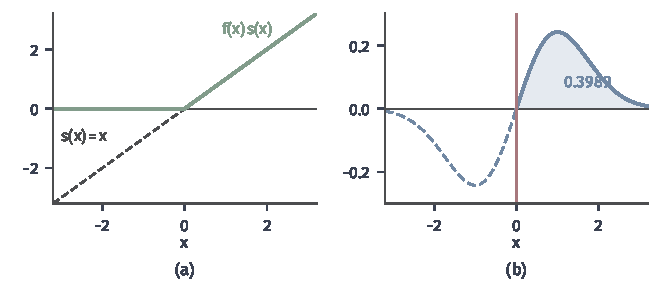
\includegraphics[width=112mm]{figures/07-probability/08-sampling-and-integration/matplotlib/pgrad-score-weights/figure.pdf}
  \caption{$X\sim\mathcal{N}(\theta,1)$在$\theta=0$处，$f(x)=\mathbf{1}_{\{x>0\}}$。(a)灰色虚线为得分$s(x)=x$，绿线为单样本估计的取值$f(x)s(x)$。(b)蓝线为$\partial_{\theta}p_{\theta}=p\,s$；红线$x=0$左侧$f=0$，这部分（虚线）不计入；右侧浅蓝面积为$\varphi(0)\approx0.3989$，等于$J'(0)$。}
  \label{fig:pgrad-score-weights}
\end{BookInlineFigure}

离散分布同样适用。$X\sim\operatorname{Bern}(\theta)$时，以计数测度为参考，$p_{\theta}(1)=\theta$，$p_{\theta}(0)=1-\theta$，得分为
\[
  s(1)=\frac{1}{\theta},\qquad s(0)=-\frac{1}{1-\theta},
\]
于是
\[
  \mathbb{E}[f(X)s(X)]=\theta\cdot\frac{f(1)}{\theta}-(1-\theta)\cdot\frac{f(0)}{1-\theta}=f(1)-f(0),
\]
正是图~\ref{fig:pgrad-bernoulli-threshold}中路径导数漏掉的那一项。

\paragraph{与重参数化在同一组样本上比较}

回到$X\sim\mathcal{N}(\mu,\sigma^{2})$、$f(x)=x^{2}$。由第~\ref{chap:information-geometry}章，两个得分分量是
\[
  s_{\mu}(x)=\frac{x-\mu}{\sigma^{2}}=\frac{\varepsilon}{\sigma},\qquad s_{\sigma}(x)=\frac{(x-\mu)^{2}-\sigma^{2}}{\sigma^{3}}=\frac{\varepsilon^{2}-1}{\sigma},
\]
其中$\varepsilon=(x-\mu)/\sigma$。用上一节同样的四个样本（$\mu=1$，$\sigma=0.5$），函数值是$f=1.3225,\ 0.2025,\ 1.9600,\ 0.6400$。$\mu$分量的单样本估计$f s_{\mu}$及其平均为
\[
  0.7935,\ -0.4455,\ 3.1360,\ -0.5120,\qquad\hat{g}_{\mu}=0.743,
\]
$\sigma$分量$f s_{\sigma}$为
\[
  -2.4069,\ 0.0851,\ -1.4112,\ -1.0752,\qquad\hat{g}_{\sigma}=-1.202 .
\]
真值是$(2,1)$，重参数化在同样的噪声上给出$(1.900,0.325)$。两种估计都无偏，但得分函数估计在这组样本上偏得更远，这不是偶然：第~\ref{sec:pgrad-variance}节会算出，在这个例子里得分函数估计的方差大得多。得分估计只利用“哪里的质量变多了”，不利用函数在样本附近怎样变化，丢掉了光滑性提供的信息。

\paragraph{支撑随参数移动}

定理~\ref{thm:pgrad-score}要求共同支撑。设$X\sim\operatorname{Unif}(0,\theta)$，$f(x)=x$，则$J(\theta)=\theta/2$，$J'(\theta)=\frac{1}{2}$。在支撑$(0,\theta)$内，$p_{\theta}(x)=1/\theta$，得分是常数$-1/\theta$。直接套用式~\eqref{eq:pgrad-score}，
\[
  \mathbb{E}_{\theta}[f(X)s_{\theta}(X)]=-\frac{1}{\theta}\mathbb{E}_{\theta}[X]=-\frac{1}{2},
\]
连符号都错了。

正确的计算要对积分上限求导。由含参积分的求导法则，
\[
  \frac{\mathrm{d}}{\mathrm{d}\theta}\int_{0}^{\theta}\frac{x}{\theta}\,\mathrm{d}x
  =\underbrace{\theta\cdot\frac{1}{\theta}}_{\text{边界}}+\int_{0}^{\theta}x\cdot\Bigl(-\frac{1}{\theta^{2}}\Bigr)\mathrm{d}x
  =1-\frac{1}{2}=\frac{1}{2}.
\]
第二项正是得分公式算出的$-\frac{1}{2}$，第一项$f(\theta)p_{\theta}(\theta^{-})=1$是新进入支撑的那一小段带来的贡献，得分只定义在旧支撑上，看不到它。第~\ref{chap:information-geometry}章用同一个均匀族说明了得分的期望在这里不为零，本例则显示加权以后漏掉的边界项可以比被计入的部分还大。

图~\ref{fig:pgrad-uniform-boundary}取$\theta=1$、$h=0.25$画出了两部分。旧支撑内$f p$从蓝线降到黄线，减少的面积是$0.1$；新增的一段$(1,1.25]$贡献$0.225$。净变化$0.125$等于$J(1.25)-J(1)$。除以$h$后两部分分别是$-0.4$与$0.9$，$h\to0$时趋于$-\frac{1}{2}$与$1$。

\begin{BookInlineFigure}
  \centering
  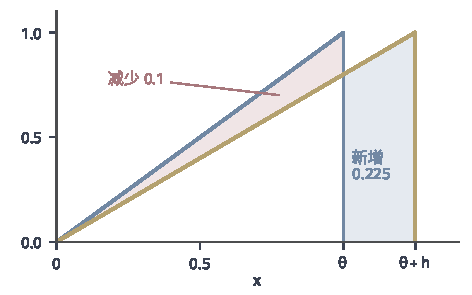
\includegraphics[width=80mm]{figures/07-probability/08-sampling-and-integration/matplotlib/pgrad-uniform-boundary/figure.pdf}
  \caption{$X\sim\operatorname{Unif}(0,\theta)$，$f(x)=x$。蓝线为$\theta=1$时的$f p_{\theta}$，黄线为$\theta+h=1.25$时的$f p_{\theta+h}$。浅红区域是旧支撑内减少的部分（面积$0.1$），得分公式只看到这一部分；浅蓝区域是新进入支撑的部分（面积$0.225$），得分公式漏掉了它。}
  \label{fig:pgrad-uniform-boundary}
\end{BookInlineFigure}

这个例子用重参数化反而没有困难：$X=\theta U$，$U\sim\operatorname{Unif}(0,1)$，路径导数$\frac{\mathrm{d}}{\mathrm{d}\theta}(\theta U)=U$，期望正是$\frac{1}{2}$。支撑的移动被样本点的移动自然地带了进去。两种方法的适用范围互补：重参数化怕函数沿路径跳跃，得分函数怕支撑随参数移动。

\subsection{未知归一化常数}
\label{sec:pgrad-score-unnormalized}

许多分布只能写到一个常数因子，例如未归一化密度取$\exp(-V_{\bm{\theta}}(x))$的形式，其中能量函数$V_{\bm{\theta}}$可以计算，而
\[
  Z_{\bm{\theta}}=\int\widetilde{p}_{\bm{\theta}}\,\mathrm{d}\nu
\]
在高维时无法直接求出。第~\ref{chap:sample-generation}章的Metropolis--Hastings采样正是为这种分布设计的：它只用到$\widetilde{p}_{\bm{\theta}}$的比值。现在要对归一化后的密度$p_{\bm{\theta}}$（即$\widetilde{p}_{\bm{\theta}}$除以$Z_{\bm{\theta}}$）下的期望求梯度，而$Z_{\bm{\theta}}$本身也随参数改变。

困难在于得分
\[
  \nabla_{\bm{\theta}}\ln p_{\bm{\theta}}=\nabla_{\bm{\theta}}\ln\widetilde{p}_{\bm{\theta}}-\nabla_{\bm{\theta}}\ln Z_{\bm{\theta}}
\]
含有$Z_{\bm{\theta}}$的导数。下面要说明，这个导数也可以写成目标分布下的期望，从而由目标样本计算。整个推导在同一个参考测度$\nu$与共同支撑$S=\{x:\widetilde{p}_{\bm{\theta}}(x)>0\}$上进行，并要求在以所论参数为中心的某个开球$U$内，每个$\bm{\theta}$都有$0<Z_{\bm{\theta}}<\infty$。需要两项交换条件：
\begin{enumerate}
  \item 归一化积分可以在积分号下求导：$\widetilde{p}_{\bm{\theta}}$在$S$上满足定理~\ref{thm:pgrad-exchange}的条件（$\mu=\nu$），于是$Z_{\bm{\theta}}$可微，梯度等于$\nabla_{\bm{\theta}}\widetilde{p}_{\bm{\theta}}$在$S$上的积分；
  \item 加权积分可以在积分号下求导：$f_{\bm{\theta}}\widetilde{p}_{\bm{\theta}}$也满足这些条件，于是加权积分
  \[
    N(\bm{\theta})=\int_{S}f_{\bm{\theta}}\widetilde{p}_{\bm{\theta}}\,\mathrm{d}\nu
  \]
  可微，梯度可在积分号下计算。
\end{enumerate}
两者缺一不可：$J=N/Z$，分子分母各自的导数都要能写成积分。

\subsubsection{得分的中心化}
\label{sec:pgrad-centering}

记未归一化密度的对数导数为
\[
  \bm{a}_{\bm{\theta}}(x)=\nabla_{\bm{\theta}}\ln\widetilde{p}_{\bm{\theta}}(x)=\frac{\nabla_{\bm{\theta}}\widetilde{p}_{\bm{\theta}}(x)}{\widetilde{p}_{\bm{\theta}}(x)},\qquad x\in S .
\]
它只用到$\widetilde{p}_{\bm{\theta}}$，可以在每个样本处计算。它和得分差多少？

\begin{lemma}[归一化常数的对数导数]
\label{lem:pgrad-logz}
在上述交换条件1下，$\bm{a}_{\bm{\theta}}(X)$在$P_{\bm{\theta}}$下可积，并且
\begin{equation}
  \nabla_{\bm{\theta}}\ln Z_{\bm{\theta}}=\mathbb{E}_{\bm{\theta}}[\bm{a}_{\bm{\theta}}(X)],
  \label{eq:pgrad-logz}
\end{equation}
从而得分是中心化的对数导数：
\begin{equation}
  \bm{s}_{\bm{\theta}}(x)=\bm{a}_{\bm{\theta}}(x)-\mathbb{E}_{\bm{\theta}}[\bm{a}_{\bm{\theta}}(X)].
  \label{eq:pgrad-centered-score}
\end{equation}
\end{lemma}

\begin{proof}
定理~\ref{thm:pgrad-exchange}的结论包含$\nabla_{\bm{\theta}}\widetilde{p}_{\bm{\theta}}$对$\nu$可积。由$\bm{a}_{\bm{\theta}}$的定义，在$S$上
\[
  \nabla_{\bm{\theta}}\widetilde{p}_{\bm{\theta}}=\widetilde{p}_{\bm{\theta}}\bm{a}_{\bm{\theta}}=Z_{\bm{\theta}}\,p_{\bm{\theta}}\bm{a}_{\bm{\theta}},
\]
所以
\[
  \mathbb{E}_{\bm{\theta}}\lVert\bm{a}_{\bm{\theta}}\rVert_{2}=\frac{1}{Z_{\bm{\theta}}}\int_{S}\lVert\nabla_{\bm{\theta}}\widetilde{p}_{\bm{\theta}}\rVert_{2}\,\mathrm{d}\nu<\infty .
\]
同一个关系与交换条件1给出
\[
  \nabla Z_{\bm{\theta}}=\int_{S}\widetilde{p}_{\bm{\theta}}\bm{a}_{\bm{\theta}}\,\mathrm{d}\nu=Z_{\bm{\theta}}\,\mathbb{E}_{\bm{\theta}}[\bm{a}_{\bm{\theta}}].
\]
因为$0<Z_{\bm{\theta}}<\infty$，两边除以$Z_{\bm{\theta}}$即得式~\eqref{eq:pgrad-logz}。最后，$\ln p_{\bm{\theta}}$与$\ln\widetilde{p}_{\bm{\theta}}$只差$\ln Z_{\bm{\theta}}$，对参数求梯度得到式~\eqref{eq:pgrad-centered-score}。
\end{proof}

这个结果的含义可以用质量的比喻说清楚。$\bm{a}_{\bm{\theta}}$记录的是未归一化质量在各位置的相对增长率，它完全可以处处为正：所有位置的质量都在增加。但概率的总量固定为$1$，归一化会把整体的增长除掉，只留下各位置相对于平均增长的差别。平均增长率按目标分布加权，就是$\mathbb{E}_{\bm{\theta}}[\bm{a}_{\bm{\theta}}]$，它等于$\ln Z_{\bm{\theta}}$的变化率。式~\eqref{eq:pgrad-centered-score}因此说：得分是相对增长率减去它的平均。中心化后的量期望为零，与第~\ref{chap:information-geometry}章得分期望为零的结论一致。

以三点分布为例。在$\{0,1,2\}$上取未归一化质量
\[
  \widetilde{p}_{\theta}(x)=h(x)\mathrm{e}^{\theta x},\qquad h=(1,2,1).
\]
此时
\[
  a_{\theta}(x)=x,\qquad Z_{\theta}=1+2\mathrm{e}^{\theta}+\mathrm{e}^{2\theta}=(1+\mathrm{e}^{\theta})^{2}.
\]
归一化后$p_{\theta}$是二项分布$\operatorname{Bin}(2,q)$，其中$q=\mathrm{e}^{\theta}/(1+\mathrm{e}^{\theta})$。直接求导得到
\[
  \frac{\mathrm{d}}{\mathrm{d}\theta}\ln Z_{\theta}=\frac{2\mathrm{e}^{\theta}}{1+\mathrm{e}^{\theta}}=2q,
\]
正是$\mathbb{E}_{\theta}[X]$，与式~\eqref{eq:pgrad-logz}一致。在$\theta=0$处，分布是$(\frac{1}{4},\frac{1}{2},\frac{1}{4})$，$a$的期望为$1$，得分是$s_{0}(x)=x-1$。

图~\ref{fig:pgrad-unnormalized}画出了这个过程。$\theta$由$0$增至$0.5$时，未归一化的三根柱子没有一根变矮；归一化以后，$x=0$处的概率从$0.25$降到约$0.14$，$x=2$处从$0.25$升到约$0.39$。$a(x)=x$全非负，减去平均$1$后才得到有正有负的得分。指数族是这个例子的一般形式：$\bm{a}_{\bm{\theta}}=\bm{T}(x)$，式~\eqref{eq:pgrad-centered-score}就是第~\ref{chap:information-geometry}章的$\bm{T}-\mathbb{E}_{\bm{\theta}}[\bm{T}]$。

\begin{BookInlineFigure}
  \centering
  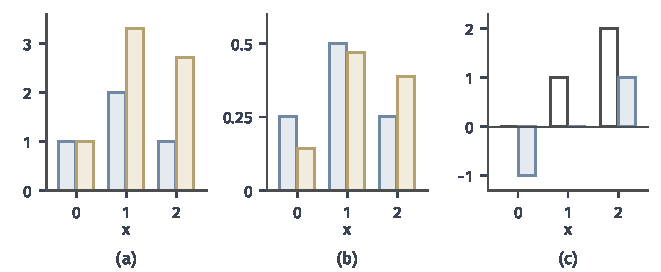
\includegraphics[width=112mm]{figures/07-probability/08-sampling-and-integration/matplotlib/pgrad-unnormalized/figure.pdf}
  \caption{$\{0,1,2\}$上的$\widetilde{p}_{\theta}(x)=h(x)\mathrm{e}^{\theta x}$，$h=(1,2,1)$。(a)未归一化质量，蓝色为$\theta=0$（总量$Z=4$），黄色为$\theta=0.5$（总量约$7.02$）；(b)归一化后的概率，质量从$x=0$移向$x=2$；(c)空心柱为$a(x)=x$，蓝色柱为$\theta=0$处的得分$s(x)=x-1$。}
  \label{fig:pgrad-unnormalized}
\end{BookInlineFigure}

\subsubsection{协方差形式}
\label{sec:pgrad-covariance}

有了中心化的得分，可以把式~\eqref{eq:pgrad-score}改写成不含$Z_{\bm{\theta}}$的形式。对标量函数$f$与向量函数$\bm{a}$，记
\[
  \operatorname{Cov}_{\bm{\theta}}(f,\bm{a})=\mathbb{E}_{\bm{\theta}}[f\bm{a}]-\mathbb{E}_{\bm{\theta}}[f]\,\mathbb{E}_{\bm{\theta}}[\bm{a}]\in\mathbb{R}^{k},
\]
它的第$j$个分量是$f$与$a_{j}$的协方差。这个定义只用到$f$、$\bm{a}$与$f\bm{a}$的可积性，不要求二阶矩。

\begin{theorem}[协方差形式的梯度]
\label{thm:pgrad-covariance}
在交换条件1与条件2下，若$f_{\bm{\theta}}$、$\nabla_{\bm{\theta}}f_{\bm{\theta}}$与$f_{\bm{\theta}}\bm{a}_{\bm{\theta}}$在$P_{\bm{\theta}}$下可积，则
\begin{equation}
  \nabla J(\bm{\theta})=\mathbb{E}_{\bm{\theta}}\bigl[\nabla_{\bm{\theta}}f_{\bm{\theta}}(X)\bigr]+\operatorname{Cov}_{\bm{\theta}}\bigl(f_{\bm{\theta}}(X),\bm{a}_{\bm{\theta}}(X)\bigr).
  \label{eq:pgrad-covariance}
\end{equation}
\end{theorem}

\begin{proof}
$J$是交换条件2中的加权积分$N$与$Z_{\bm{\theta}}$之比。由交换条件2，
\[
  \nabla N=\int_{S}\bigl(\nabla_{\bm{\theta}}f_{\bm{\theta}}+f_{\bm{\theta}}\bm{a}_{\bm{\theta}}\bigr)\widetilde{p}_{\bm{\theta}}\,\mathrm{d}\nu=Z_{\bm{\theta}}\,\mathbb{E}_{\bm{\theta}}\bigl[\nabla_{\bm{\theta}}f_{\bm{\theta}}+f_{\bm{\theta}}\bm{a}_{\bm{\theta}}\bigr],
\]
其中拆成两个期望用到了所设的可积性。由交换条件1与引理~\ref{lem:pgrad-logz}的证明，$\nabla Z_{\bm{\theta}}$等于$Z_{\bm{\theta}}\mathbb{E}_{\bm{\theta}}[\bm{a}_{\bm{\theta}}]$。商的求导法则给出
\[
  \nabla J=\frac{\nabla N}{Z_{\bm{\theta}}}-\frac{N}{Z_{\bm{\theta}}}\cdot\frac{\nabla Z_{\bm{\theta}}}{Z_{\bm{\theta}}}
  =\mathbb{E}_{\bm{\theta}}\bigl[\nabla_{\bm{\theta}}f_{\bm{\theta}}+f_{\bm{\theta}}\bm{a}_{\bm{\theta}}\bigr]-\mathbb{E}_{\bm{\theta}}[f_{\bm{\theta}}]\,\mathbb{E}_{\bm{\theta}}[\bm{a}_{\bm{\theta}}],
\]
整理即得式~\eqref{eq:pgrad-covariance}。
\end{proof}

逐个分量看，第$j$个分量的第二项是$\operatorname{Cov}_{\bm{\theta}}(f,a_{j})$。沿第$j$个参数方向，未归一化质量在$x$处按相对速率$a_{j}(x)$增长。若增长得快的地方恰好是$f$大的地方，协方差为正，期望上升；若两者无关，协方差为零，质量的增长只是整体放大，归一化后什么也没有改变。给$a_{j}$加上任何常数（各处等速增长）都不改变协方差。$\ln Z_{\bm{\theta}}$的导数正是以这种方式计入的：协方差中减去的$\mathbb{E}[f]\mathbb{E}[a_{j}]$就是那一项，而计算它只需要目标样本，不需要知道$Z_{\bm{\theta}}$。

在三点分布的例子中取$f(x)=x^{2}$，与参数无关。在$\theta=0$处，
\[
  \mathbb{E}_{0}[f]=\tfrac{0+2+4}{4}=1.5,\quad\mathbb{E}_{0}[a]=1,\quad\mathbb{E}_{0}[fa]=\mathbb{E}_{0}[X^{3}]=\tfrac{0+2+8}{4}=2.5,
\]
于是$J'(0)=\operatorname{Cov}_{0}(X^{2},X)=2.5-1.5=1$。用闭式核对：$X\sim\operatorname{Bin}(2,q)$时$J=\mathbb{E}[X^{2}]=2q+2q^{2}$，而$\mathrm{d}q/\mathrm{d}\theta=q(1-q)$，所以
\[
  J'(\theta)=(2+4q)\,q(1-q),
\]
在$q=\frac{1}{2}$处等于$4\cdot\frac{1}{4}=1$，两种算法一致。

\subsubsection{样本估计}
\label{sec:pgrad-cov-sample}

式~\eqref{eq:pgrad-covariance}中的期望与协方差都要用目标样本估计。设$X_{1},\dots,X_{n}$（$n\geq2$）独立同分布于$P_{\bm{\theta}}$，记$F_{i}=f_{\bm{\theta}}(X_{i})$，$\bm{A}_{i}=\bm{a}_{\bm{\theta}}(X_{i})$，$\bar{F}$与$\bar{\bm{A}}$为样本平均。以样本平均作中心的协方差估计取分母$n-1$：
\begin{equation}
  \hat{\bm{C}}_{n}=\frac{1}{n-1}\sum_{i=1}^{n}(F_{i}-\bar{F})(\bm{A}_{i}-\bar{\bm{A}}).
  \label{eq:pgrad-cov-estimator}
\end{equation}
梯度的估计是$\frac{1}{n}\sum_{i}\nabla_{\bm{\theta}}f_{\bm{\theta}}(X_{i})+\hat{\bm{C}}_{n}$。

为什么是$n-1$？展开乘积，
\[
  \sum_{i=1}^{n}(F_{i}-\bar{F})(\bm{A}_{i}-\bar{\bm{A}})=\sum_{i=1}^{n}F_{i}\bm{A}_{i}-n\bar{F}\bar{\bm{A}} .
\]
第一项的期望是$n\,\mathbb{E}[f\bm{a}]$。第二项里
\[
  \bar{F}\bar{\bm{A}}=\frac{1}{n^{2}}\sum_{i=1}^{n}\sum_{j=1}^{n}F_{i}\bm{A}_{j},
\]
其中$n$个$i=j$的项期望为$\mathbb{E}[f\bm{a}]$，其余$n(n-1)$项由独立性期望为$\mathbb{E}[f]\mathbb{E}[\bm{a}]$，所以
\[
  \mathbb{E}\bigl[n\bar{F}\bar{\bm{A}}\bigr]=\mathbb{E}[f\bm{a}]+(n-1)\,\mathbb{E}[f]\,\mathbb{E}[\bm{a}].
\]
两式相减，
\[
  \mathbb{E}\Bigl[\sum_{i=1}^{n}(F_{i}-\bar{F})(\bm{A}_{i}-\bar{\bm{A}})\Bigr]=(n-1)\operatorname{Cov}_{\bm{\theta}}(f,\bm{a}).
\]
用样本平均作中心时，每个样本都参与了它自己的中心，这使乘积系统地偏小，损失恰好是一个样本的份额。除以$n-1$得到无偏估计；除以$n$则期望为$\frac{n-1}{n}\operatorname{Cov}_{\bm{\theta}}(f,\bm{a})$，小样本时偏差明显。推导只用到独立同分布和$f$、$\bm{a}$、$f\bm{a}$的可积性。

用三点分布在$\theta=0$处手算一次。由逆变换，累积概率的分点是$0.25$与$0.75$，均匀数$u=0.37,0.80,0.15,0.62$给出
\[
  X=1,\ 2,\ 0,\ 1,\qquad F=1,\ 4,\ 0,\ 1,\qquad A=1,\ 2,\ 0,\ 1 .
\]
样本平均为$\bar{F}=1.5$、$\bar{A}=1$，中心化后的乘积依次是
\[
  (-0.5)\cdot0,\quad2.5\cdot1,\quad(-1.5)\cdot(-1),\quad(-0.5)\cdot0,
\]
和为$4$。除以$n-1=3$得$\hat{C}_{4}=1.333$，除以$n=4$得$1$。真值是$1$；这一组样本恰好让有偏的版本更接近真值，但平均而言它偏小$25\%$。图~\ref{fig:pgrad-cov-bias}用大量重复显示了两种分母的平均行为。

\begin{BookInlineFigure}
  \centering
  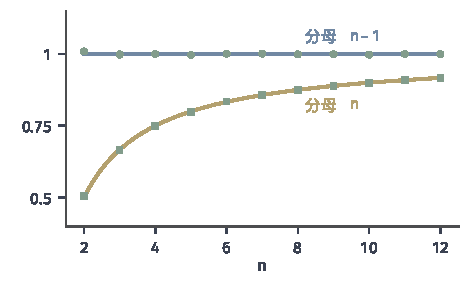
\includegraphics[width=80mm]{figures/07-probability/08-sampling-and-integration/matplotlib/pgrad-cov-bias/figure.pdf}
  \caption{三点分布$p_{0}=(\frac{1}{4},\frac{1}{2},\frac{1}{4})$上$\operatorname{Cov}(X^{2},X)=1$的两种样本估计。蓝线与绿色圆点：分母$n-1$，期望恒为$1$；黄线与绿色方块：分母$n$，期望$(n-1)/n$。线为精确期望，点为每个$n$重复$40000$次（固定种子）的平均。}
  \label{fig:pgrad-cov-bias}
\end{BookInlineFigure}

这个无偏保证依赖独立同分布。未归一化目标的样本通常来自MCMC，链上的样本相关，而且从一般初值出发时各时刻的分布还不是$P_{\bm{\theta}}$。这时推导中“$i\neq j$的项期望为$\mathbb{E}[f]\mathbb{E}[\bm{a}]$”不再成立，$n-1$分母不再修正什么，有限样本偏差由链的初值与相关性决定，要按第~\ref{sec:pgrad-approx}节与第~\ref{chap:monte-carlo-integration-error}章检查。若改用自归一化重要性采样的加权样本，加权协方差是两个随机量之比，有限样本下一般有偏，要按第~\ref{chap:variance-reduction}章对比值估计的分析检查。无偏只是一阶的性质，估计的二阶矩是否有限、波动有多大，是下一节的问题。
